\documentclass[letterpaper]{article}
\usepackage[utf8]{inputenc}
\usepackage[margin=0.3in,footskip=0.25in]{geometry}

% import tikz library
\usepackage{tikz}
\usetikzlibrary{shapes, arrows}

% Global adjustment factors
\newcommand\x{-2.3cm}
\newcommand\y{-0.8cm}

% define the shapes we want to use
\tikzstyle{startstop} = [ellipse, minimum width=2.5cm, minimum height=0.8cm, draw=black, fill=red!20, text centered, text width=12em]
\tikzstyle{process} = [rectangle, minimum width=0.5cm, minimum height=0.5cm, text centered, draw=black, fill=blue!20, text width=13em]
\tikzstyle{decision} = [diamond, minimum width=0cm, minimum height=0.0cm, text centered, draw=black, fill=yellow!20, text width=11.414em, aspect=2]
\tikzstyle{cont} = [circle, minimum width=1cm, minimum height=1cm, text centered, draw=black, fill=green!20]

\tikzstyle{ss_legend} =[ellipse, minimum width=0.5cm, minimum height=0.3cm, draw=black, fill=red!20]
\tikzstyle{process_legend} = [rectangle, minimum width=0.5cm, minimum height=0.5cm, draw=black, fill=blue!20]
\tikzstyle{decision_legend} = [diamond, minimum width=0cm, minimum height=0.0cm, draw=black, fill=yellow!20]
\tikzstyle{cont_legend} = [circle, minimum width=0.5cm, minimum height=0.5cm, draw=black, fill=green!20]

\tikzstyle{line} = [draw, -latex']


\begin{document}
    
    \scriptsize
    \begin{center}
        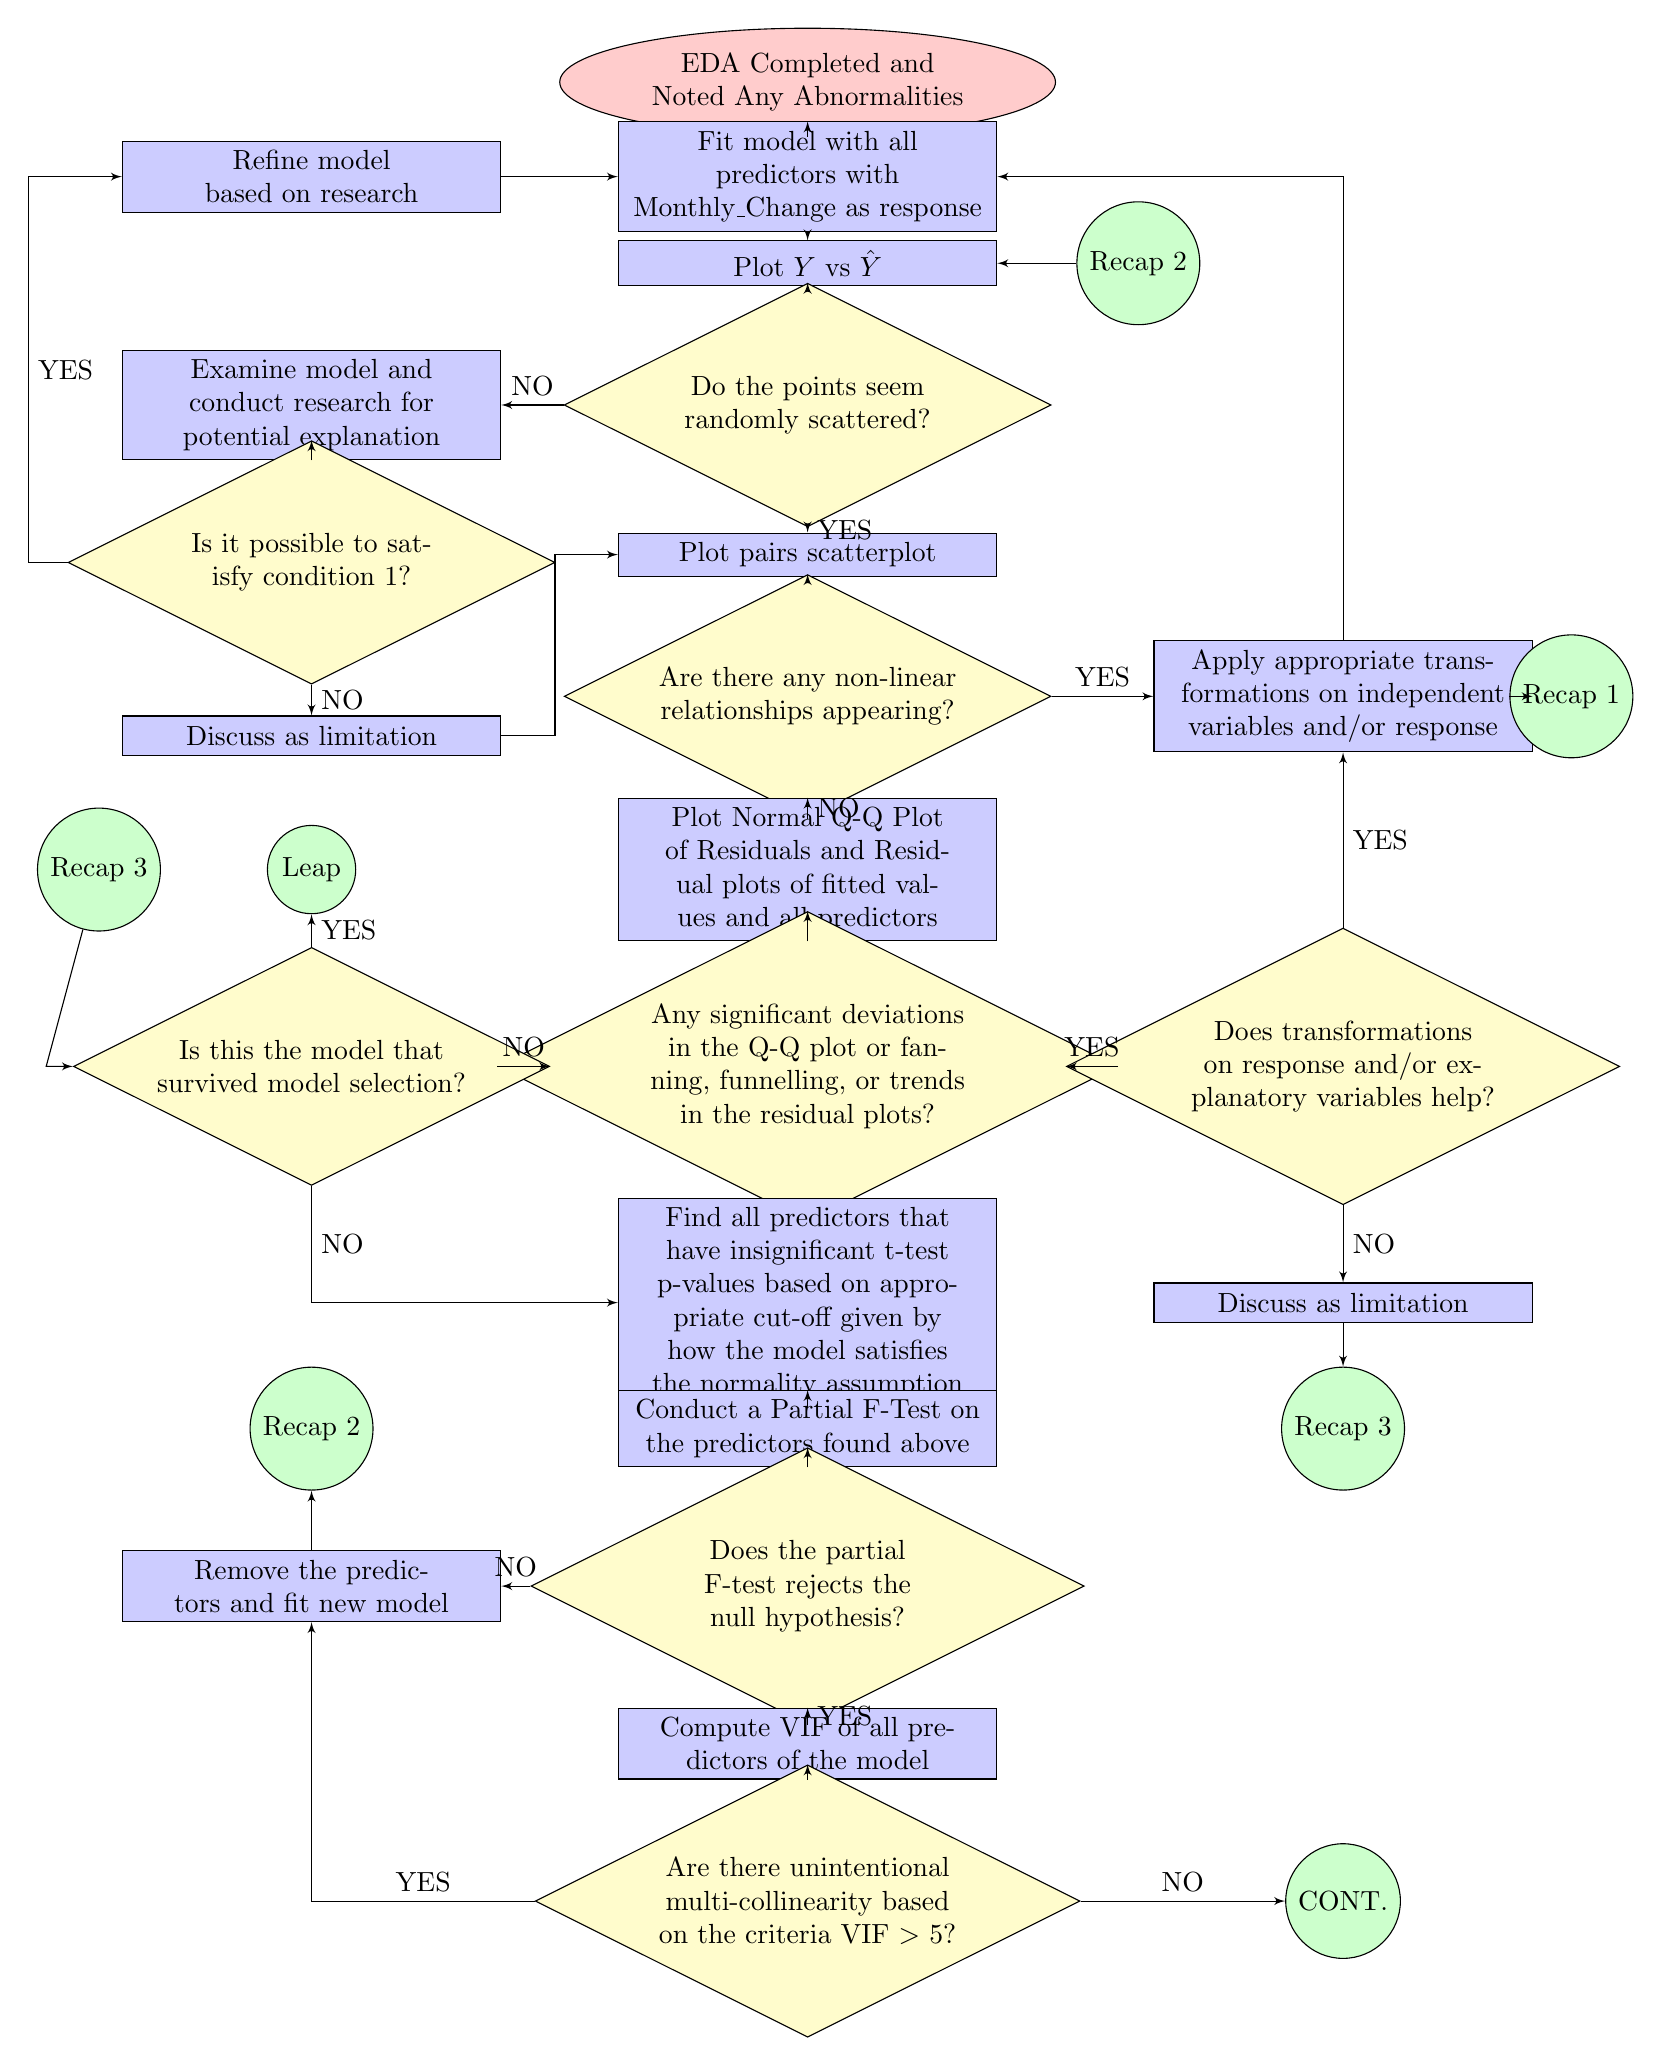
\begin{tikzpicture}[node distance=1.2cm, auto]
            
            % Nodes of flowchart
            % Main line
            \node (start) [startstop] {EDA Completed and Noted Any Abnormalities};
            \node (pro_1) [process, below of=start] {Fit model with all predictors with Monthly$\_$Change as response};
            \node (pro_7) [process, below of=pro_1, yshift=0.1cm] {Plot $Y$ vs $\hat{Y}$};
            \node (dec_1) [decision, below of=pro_7, yshift=-0.6cm] {Do the points seem randomly scattered?};
            \node (pro_2) [process, below of=dec_1, yshift=-0.7cm] {Plot pairs scatterplot};
            \node (dec_2) [decision, below of=pro_2, yshift=-0.6cm] {Are there any non-linear relationships appearing?};
            \node (pro_3) [process, below of=dec_2, yshift=-1cm] {Plot Normal Q-Q Plot of Residuals and Residual plots of fitted values and all predictors};
            \node (dec_3) [decision, below of=pro_3, yshift=-1.3cm] {Any significant deviations in the Q-Q plot or fanning, funnelling, or trends in the residual plots?};
            \node (pro_4) [process, below of=dec_3, yshift=-1.8cm] {Find all predictors that have insignificant t-test p-values based on appropriate cut-off given by how the model satisfies the normality assumption};
            \node (pro_5) [process, below of=pro_4, yshift=-0.4cm] {Conduct a Partial F-Test on the predictors found above};
            \node (dec_4) [decision, below of=pro_5, yshift=-0.8cm] {Does the partial F-test rejects the null hypothesis?};
            \node (pro_11) [process, below of=dec_4, yshift=-0.8cm] {Compute VIF of all predictors of the model};
            \node (dec_7) [decision, below of=pro_11, yshift=-0.8cm] {Are there unintentional multi-collinearity based on the criteria VIF $>$ 5?};
            
            % Left line
            \node (pro_8) [process, left of=pro_1, xshift=-5.1cm] {Refine model based on research};
            \node (pro_9) [process, left of=dec_1, xshift=-5.1cm] {Examine model and conduct research for potential explanation};
            \node (dec_5) [decision, below of=pro_9, yshift=-0.8cm] {Is it possible to satisfy condition 1?};
            \node (pro_10) [process, below of=dec_5, yshift=-1cm] {Discuss as limitation};
            \node (pro_6) [process, left of=dec_4, xshift=-5.1cm] {Remove the predictors and fit new model};
            \node (recap2_1) [cont, left of=pro_5, xshift=-5.1cm] {Recap 2};
            \node (dec_x) [decision, left of=dec_3, xshift=-5.1cm] {Is this the model that survived model selection?};
            \node (leap) [cont, left of=pro_3, xshift=-5.1cm] {Leap}; 
            \node (recap3_2) [cont, left of=leap, xshift=-1.5cm] {Recap 3};
            
            
            % Right line
            \node (pro_12) [process, right of=dec_2, xshift=5.6cm] {Apply appropriate transformations on independent variables and/or response};
            \node (dec_6) [decision, right of=dec_3, xshift=5.6cm] {Does transformations on response and/or explanatory variables help?};
            \node (pro_13) [process, right of=pro_4, xshift=5.6cm] {Discuss as limitation};
            \node (recap3_1) [cont, below of=pro_13, yshift=-0.4cm] {Recap 3};
            
            
            % Other
            \node (recap1_2) [cont, right of=pro_12, xshift=1.7cm] {Recap 1};
            \node (recap2_2) [cont, right of=pro_7, xshift=3cm] {Recap 2};
            \node (cont) [cont, right of=dec_7, xshift=5.6cm] {CONT.};
            
            % Draw lines
            % Main line
            \path [line] (start) -- (pro_1);
            \path [line] (pro_1) -- (pro_7);
            \path [line] (pro_7) -- (dec_1);
            \path [line] (dec_1) -- node[anchor=west] {YES} (pro_2);
            \path [line] (pro_2) -- (dec_2);
            \path [line] (dec_2) -- node[anchor=west] {NO} (pro_3);
            \path [line] (pro_3) -- (dec_3);
            \path [line] (dec_3) -- node[anchor=south] {NO} (dec_x);
            \path [line] (dec_4) -- node[anchor=south] {NO} (pro_6);
            \path [line] (pro_4) -- (pro_5);
            \path [line] (pro_5) -- (dec_4);
            \path [line] (dec_4) -- node[anchor=west] {YES} (pro_11);
            \path [line] (pro_11) -- (dec_7);
            \path [line] (dec_7) -| node[pos=0.25, anchor=south] {YES} (pro_6);
            
            % Left line
            \path [line] (pro_8) -- (pro_1);
            \path [line] (pro_9) -- (dec_5);
            \path [line] (dec_1) -- node[anchor=south] {NO} (pro_9);
            \path [line] (dec_5) -- node[anchor=west] {NO} (pro_10);
            \path [line] (dec_5) --  ([xshift=-0.5cm] dec_5.west) |- node[pos=0.25, anchor=west] {YES}  (pro_8);
            \path [line] (pro_10) -| ([xshift=-0.8cm] pro_2.west) -- (pro_2);
            \path [line] (pro_6) -- (recap2_1);
            \path [line] (dec_x) |- node[pos=0.25, anchor=west] {NO} (pro_4);
            \path [line] (dec_x) -- node[pos=0.5, anchor=west] {YES} (leap);
            \path [line] (recap3_2) -- ([xshift=-0.34cm] dec_x.west) -- (dec_x);
            
            % Right line
            \path [line] (pro_12) |- (pro_1);
            \path [line] (dec_2) -- node[anchor=south] {YES} (pro_12);
            \path [line] (dec_3) -- node[anchor=south] {YES} (dec_6);
            \path [line] (dec_6) -- node[anchor=west] {YES} (pro_12);
            \path [line] (dec_6) -- node[anchor=west] {NO} (pro_13);
            \path [line] (pro_13) -- (recap3_1);
            
            % Other
            \path [line] (recap1_2) -- (pro_12);
            \path [line] (recap2_2) -- (pro_7);
            \path [line] (dec_7) -- node[anchor=south] {NO} (cont);
        \end{tikzpicture}
        
        \newpage 
        
        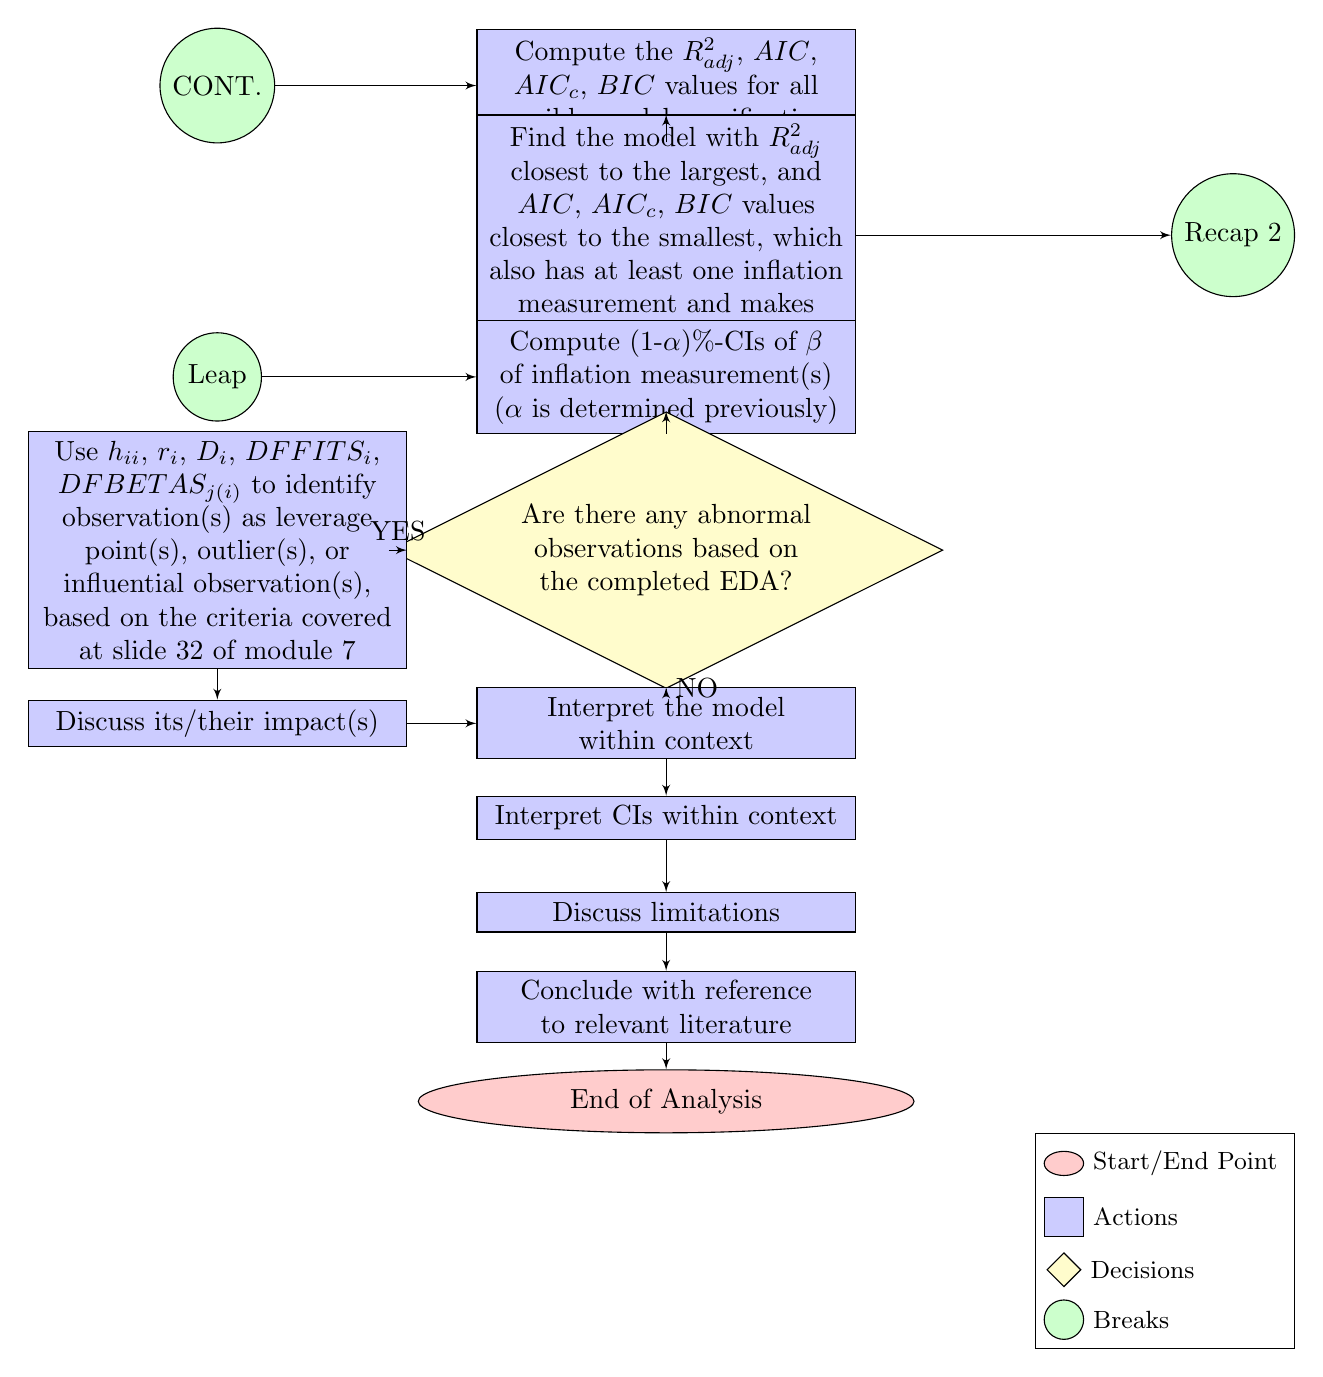
\begin{tikzpicture}[node distance=1.2cm, auto]
            % Draw nodes
            % Main line
            \node (pro1) [process] {Compute the $R^2_{adj}$, $AIC$, $AIC_c$, $BIC$ values for all possible model specifications};
            \node (pro2) [process, below of=pro1, yshift=-0.7cm] {Find the model with $R^2_{adj}$ closest to the largest, and $AIC$, $AIC_c$, $BIC$ values closest to the smallest, which also has at least one inflation measurement and makes the most contextual sense};
            \node (pro3) [process, below of=pro2, yshift=-0.6cm] {Compute (1-$\alpha$)\%-CIs of $\beta$ of inflation measurement(s) ($\alpha$ is determined previously)};
            \node (dec1) [decision, below of=pro3, yshift=-1cm] {Are there any abnormal observations based on the completed EDA?};
            \node (pro6) [process, below of=dec1, yshift=-1cm] {Interpret the model within context};
            \node (pro7) [process, below of=pro6] {Interpret CIs within context};
            \node (pro8) [process, below of=pro7] {Discuss limitations};
            \node (pro9) [process, below of=pro8] {Conclude with reference to relevant literature};
            \node (stop) [startstop, below of=pro9] {End of Analysis};
            
            % Right line
            \node (recap2) [cont, right of=pro2, xshift=6cm] {Recap 2};
            
            % Left line
            \node (cont) [cont, left of=pro1, xshift=-4.5cm] {CONT.};
            \node (leap) [cont, left of=pro3, xshift=-4.5cm] {Leap};
            \node (pro4) [process, left of=dec1, xshift=-4.5cm] {Use $h_{ii}$, $r_i$, $D_i$, $DFFITS_i$, $DFBETAS_{j(i)}$ to identify observation(s) as leverage point(s), outlier(s), or influential observation(s), based on the criteria covered at slide 32 of module 7};
            \node (pro5) [process, left of=pro6, xshift=-4.5cm] {Discuss its/their impact(s)};
            
            % Draw lines
            % Main
            \path [line] (pro1) -- (pro2);
            \path [line] (pro2) -- (recap2);
            \path [line] (pro3) -- (dec1);
            \path [line] (dec1) -- node[anchor=south] {YES} (pro4);
            \path [line] (dec1) -- node[anchor=west] {NO} (pro6);
            \path [line] (pro6) -- (pro7);
            \path [line] (pro7) -- (pro8);
            \path [line] (pro8) -- (pro9);
            \path [line] (pro9) -- (stop);
            
            % Left line
            \path [line] (pro4) -- (pro5);
            \path [line] (pro5) -- (pro6);
            
            % Other
            \path [line] (cont) -- (pro1);
            \path [line] (leap) -- (pro3);
            
            \small{
            \matrix [draw, below left] at (current bounding box.south east) {
                \node (l1) [ss_legend, label=right:Start/End Point] {}; \\
                \node (l2) [process_legend, label=right:Actions, below of=l1, yshift=0.9cm] {}; \\
                \node (l3) [decision_legend, label=right:Decisions, below of=l2, yshift=1.2cm] {}; \\
                \node (l4) [cont_legend, label=right:Breaks, below of=l3, yshift=1.2cm] {}; \\
            };
            }
        \end{tikzpicture}
        
        
    \end{center}
\end{document}
